\documentclass[12pt]{article}
\usepackage[utf8]{inputenc}
\usepackage{listings}
\usepackage{graphicx}

\title{Problemas no SGI}
\author{Henrique Henriques}
\date{Última Atualização: 26 de Setembro de 2023}

\begin{document}

\maketitle

\section{Introdução}
Este documento tem como objetivo explicar alguns dos problemas comuns enfrentados no SGI e suas respectivas soluções.

\section{Problemas e Soluções}
\subsection{Múltiplos usuários "meuovo" na tabela de usuários}
\subsubsection{Descrição}
A tabela de usuários do aplicativo contém múltiplas instâncias de usuários com o nome "meuovo", causando confusão e potenciais erros.

\subsubsection{Solução}
Execute o seguinte código SQL para remover as entradas duplicadas:
    \begin{lstlisting}[language=SQL, breaklines=true]
DELETE FROM basedb.aspnetusers WHERE Id='00a71569-0a65-4b3c-83e7-6fa48e6f9a92';
DELETE FROM basedb.aspnetusers WHERE Id='019f9312-211b-4ca8-b86f-f272b3e7459c';
DELETE FROM basedb.aspnetusers WHERE Id='03d60c0b-3dad-4c14-bcc8-d4d02c35933d';
DELETE FROM basedb.aspnetusers WHERE Id='04f7a469-7bf2-4f79-b997-c497eebe07c9';
DELETE FROM basedb.aspnetusers WHERE Id='08b5b9c5-312f-4d2a-938f-6949d9771d84';
DELETE FROM basedb.aspnetusers WHERE Id='1338ca6b-a60e-4f99-8e76-4052485f553e';
DELETE FROM basedb.aspnetusers WHERE Id='188bddd8-ef79-4fa9-91a6-21a458297edd';
DELETE FROM basedb.aspnetusers WHERE Id='2273e4d7-41f1-4688-a9ed-72ce17210d0c';
DELETE FROM basedb.aspnetusers WHERE Id='22a3113a-180b-42de-882a-cf12221a8842';
DELETE FROM basedb.aspnetusers WHERE Id='235d9f66-4ec2-4aec-a402-06ae4e5eb5e7';
DELETE FROM basedb.aspnetusers WHERE Id='24240ca3-f154-494f-9f5c-b4bb39591aca';
DELETE FROM basedb.aspnetusers WHERE Id='26144b62-d636-4b11-bc6d-dc36f165224e';
DELETE FROM basedb.aspnetusers WHERE Id='2802da02-546f-4e23-a105-e7374359509e';
DELETE FROM basedb.aspnetusers WHERE Id='28dcf1c3-1b6b-4583-9656-51c8048a1fe1';
DELETE FROM basedb.aspnetusers WHERE Id='29adbf51-4658-40bc-b512-12432ab55b9e';
DELETE FROM basedb.aspnetusers WHERE Id='2ce41d80-07f4-4fc4-9299-a968422a1e5b';
DELETE FROM basedb.aspnetusers WHERE Id='2ceccc40-8595-4682-99ac-c330157ef1c0';
DELETE FROM basedb.aspnetusers WHERE Id='305c23d0-dbed-410d-9a1c-bbde4d5f40b6';
DELETE FROM basedb.aspnetusers WHERE Id='318072b9-cf7b-4877-84f5-27d2031528ea';
DELETE FROM basedb.aspnetusers WHERE Id='31f67a28-5998-4af8-9511-661aeb7627df';
DELETE FROM basedb.aspnetusers WHERE Id='36249c53-d925-485e-9518-52f395b0d4bb';
DELETE FROM basedb.aspnetusers WHERE Id='3920c0f3-e00f-4e63-9cd2-48f57ae69048';
DELETE FROM basedb.aspnetusers WHERE Id='3d4d88e7-3c68-4013-a5ba-eab84ff0b31a';
DELETE FROM basedb.aspnetusers WHERE Id='443a83d1-7825-4d21-a1ab-4f35eff72d10';
DELETE FROM basedb.aspnetusers WHERE Id='46295a08-ddc5-41cd-a972-a0ba180c24bb';
DELETE FROM basedb.aspnetusers WHERE Id='4ae93cc8-4e6f-45dd-8e0a-bb4a645f638a';
DELETE FROM basedb.aspnetusers WHERE Id='509eb147-887b-47a8-ac88-80f540c18622';
DELETE FROM basedb.aspnetusers WHERE Id='52589239-d881-4088-8a84-150f5775d034';
DELETE FROM basedb.aspnetusers WHERE Id='54650303-761a-421a-9a0c-2faabbe4c718';
DELETE FROM basedb.aspnetusers WHERE Id='550c8276-11f6-4e92-8845-8b5b8d8f0008';
DELETE FROM basedb.aspnetusers WHERE Id='559b30b1-7f85-47a0-83ba-f70e9c3d35aa';
DELETE FROM basedb.aspnetusers WHERE Id='586ce5f7-3add-4a88-b4c5-9ec94bd79d70';
DELETE FROM basedb.aspnetusers WHERE Id='622b706d-0515-42d4-a4f3-f03e0990daca';
DELETE FROM basedb.aspnetusers WHERE Id='63ab7bbe-aeaf-4d5e-982b-e2c9ea73938d';
DELETE FROM basedb.aspnetusers WHERE Id='679c1fc3-796a-4cc7-b3b7-03b4bf0e9d13';
DELETE FROM basedb.aspnetusers WHERE Id='68f566ae-f32e-4051-be4b-12cc1a23ec01';
DELETE FROM basedb.aspnetusers WHERE Id='6ea899e6-f119-4202-b60a-df1691472fa4';
DELETE FROM basedb.aspnetusers WHERE Id='791a373d-d8fe-4849-b301-72c67383ed58';
DELETE FROM basedb.aspnetusers WHERE Id='7d597964-66d6-45b5-98da-d71c01b12f67';
DELETE FROM basedb.aspnetusers WHERE Id='7e25ab63-79c3-457e-9d06-7f09b164f132';
DELETE FROM basedb.aspnetusers WHERE Id='8b5fa2e7-56f2-4d84-aab7-78c52ca4c1db';
DELETE FROM basedb.aspnetusers WHERE Id='99661c11-05e6-4e14-b0bc-57d3e458ebcb';
DELETE FROM basedb.aspnetusers WHERE Id='9f34d20c-030e-4389-80a9-b49f3c43143b';
DELETE FROM basedb.aspnetusers WHERE Id='a7fc237a-26c3-47ac-a9e4-b8bed7fd3824';
DELETE FROM basedb.aspnetusers WHERE Id='a9604074-e186-4c33-ab93-49ab34e39ce1';
DELETE FROM basedb.aspnetusers WHERE Id='ae2dac6e-1e08-416c-851b-20071a792672';
DELETE FROM basedb.aspnetusers WHERE Id='b1f6b3f5-e3de-44f3-8932-fbd7a53f6b3c';
DELETE FROM basedb.aspnetusers WHERE Id='b251f477-e9aa-41b8-a939-1fd0374dc310';
DELETE FROM basedb.aspnetusers WHERE Id='b7f68914-c6bf-42c8-a710-43376e8a8586';
DELETE FROM basedb.aspnetusers WHERE Id='ba5654c9-46ea-4c1b-b67a-c56dd9bcca5c';
DELETE FROM basedb.aspnetusers WHERE Id='bc95723d-9bad-4fa8-bb63-1ced6ffc5c80';
DELETE FROM basedb.aspnetusers WHERE Id='c1496f0b-7ce7-42ca-8c49-05673eceee83';
DELETE FROM basedb.aspnetusers WHERE Id='c36ea7a1-87d7-4a7f-93d6-2a347de37b5d';
DELETE FROM basedb.aspnetusers WHERE Id='c590f22c-3a09-423d-bf28-baadb449a369';
DELETE FROM basedb.aspnetusers WHERE Id='c5d16edf-083f-4564-a6cc-1751c98ecc3b';
DELETE FROM basedb.aspnetusers WHERE Id='d3e8ae55-5f78-41e9-a9cf-a1d6a8c2ec59';
DELETE FROM basedb.aspnetusers WHERE Id='dabba46c-a69d-4676-a8e4-8a6c5598ab76';
DELETE FROM basedb.aspnetusers WHERE Id='dbf4647d-5783-405d-8655-79f9369c4c8e';
DELETE FROM basedb.aspnetusers WHERE Id='dd51fb00-b8eb-4317-9a68-a7384caa3d3b';
DELETE FROM basedb.aspnetusers WHERE Id='de520546-e0f8-4933-880a-a4fb947a3684';
DELETE FROM basedb.aspnetusers WHERE Id='df004375-f0e6-46c3-b1b4-8c8660705c75';
DELETE FROM basedb.aspnetusers WHERE Id='dfdedcc3-851e-4975-a743-9bc8a91078ef';
DELETE FROM basedb.aspnetusers WHERE Id='e2a0a830-4a98-4655-8735-0bd4e8264622';
DELETE FROM basedb.aspnetusers WHERE Id='eb54d322-834a-4e0e-8657-51715bd41ecb';
DELETE FROM basedb.aspnetusers WHERE Id='ebdad914-3d12-48f3-942c-49def121dcd7';
DELETE FROM basedb.aspnetusers WHERE Id='ec6d0124-b63c-40fb-85e6-c0e83518ac4e';
DELETE FROM basedb.aspnetusers WHERE Id='ecc91b22-e8e8-457f-8794-bedb713b5d01';
DELETE FROM basedb.aspnetusers WHERE Id='ecd12bba-e0c8-472c-8d2a-9a54b9a40873';
DELETE FROM basedb.aspnetusers WHERE Id='f15d6bf2-ccea-4152-ac88-7c8e5c191f1f';
DELETE FROM basedb.aspnetusers WHERE Id='f2caff3f-5c15-4185-aa49-d5b870b17b80';
DELETE FROM basedb.aspnetusers WHERE Id='f475a734-79b4-4f5c-a95d-187e3d4cb3e9';
DELETE FROM basedb.aspnetusers WHERE Id='f539b696-c3cd-47ea-81c1-40b63e6f7435';
\end{lstlisting}

\subsubsection{Observação}
Certifique-se de que nenhum usuário importante tenha sido removido inadvertidamente.

\subsection{Unable to cast object of type 'System.DBNull' to type 'System.Boolean'}
\subsubsection{Descrição}
Alguma coluna que deveria conter valores booleanos está com valores nulos.

\subsubsection{Solução}
Atualize toda a coluna Ancora na tabela Prospeccao para 0:
\begin{lstlisting}[language=SQL]
UPDATE Prospeccao SET Ancora = 0;
\end{lstlisting}

\subsection{Unable to cast object of Type 'System.String' to type 'System.Int32'}
\subsubsection{Descrição}
Incompatibilidade de tipos entre a base de dados e o código.

\subsubsection{Solução}
Verifique a compatibilidade de tipos entre o banco de dados e o código. Atualize o schema do banco de dados conforme necessário.

\subsection{Gráfico de Participação Lateral carrega de forma infinita}
\subsubsection{Descrição}
A rota não está retornando os dados esperados ou retorna nulo.

\subsubsection{Solução}
Verifique a rota pela URL: \texttt{/Participacao/PuxarDadosParticipacao}.

\subsection{Uncaught typeerror l[0] is undefined ao clicar em algum select}

\subsubsection{Descrição}
Ao clicar em um campo de seleção multipla select2, um erro misterioso de TypeError aparece no console do navegador e o select não funciona.

\begin{figure}[h!]
    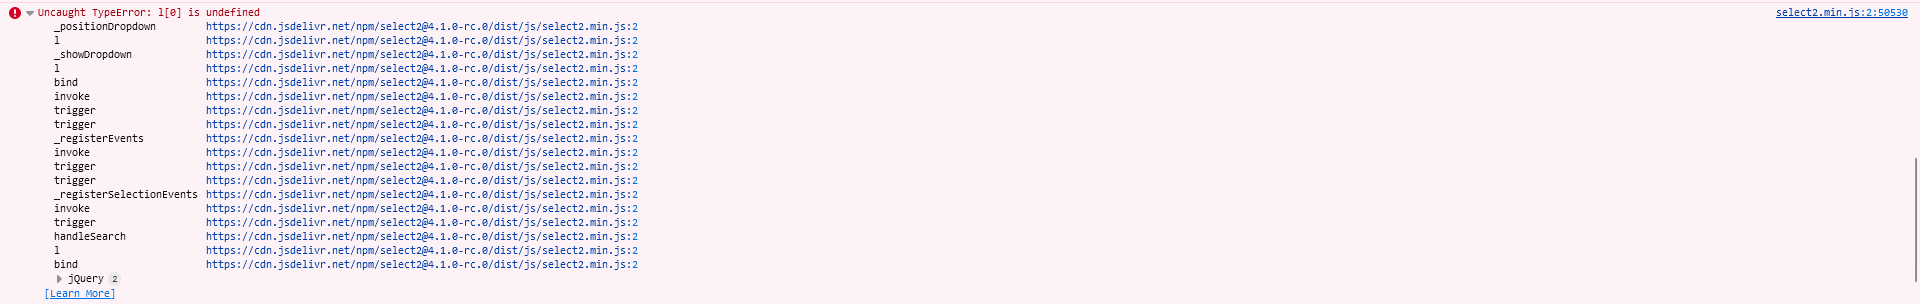
\includegraphics[width=\linewidth]{Imagens/typeerrorselect.png}
    \caption{Erro no Console do Firefox}
\end{figure}

\subsubsection{Solução}
Verifique se o código que atrela o dropdown do modal está encontrando o elementoPai no método gerarOpcoesSelect

\subsection{Ao clicar em botão que deveria acessar modal, modal não abre e um erro JS misterioso é lançado no console}
\subsubsection{Descrição}
Ao tentar acessar um modal, observa-se um erro tipo "Uncaught TypeError: this.\textunderscore config is undefined"

\begin{figure}[h!]
	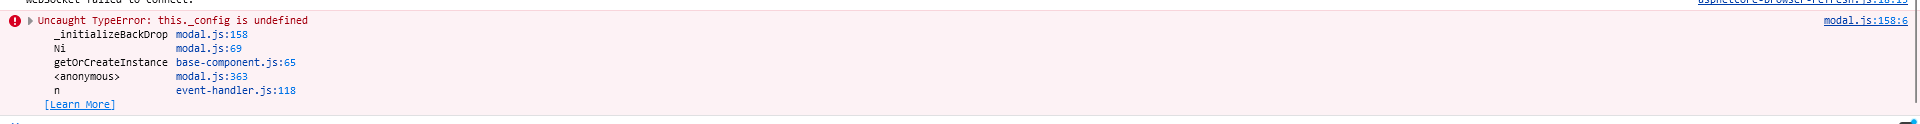
\includegraphics[width=\linewidth]{Imagens/modalerror.png}
	\caption{Erro no Console do Firefox}
\end{figure}

\subsubsection{Solução}
Verifique se o identificador do modal bate com o botão ou script que está tentando spawnar o modal. Exemplo botão tem id="meumodal" e modal tem id="modalbacana"

\section{Soluções Gerais}
\subsection{Resetar o banco local}
Restaurar o banco local a partir de um backup recente pode ser uma solução rápida e eficaz.

\subsection{Resetar as mudanças realizadas no Git}
Utilizar comandos como \texttt{git stash} pode reverter problemas de código recentes.

\end{document}
